\documentclass[tikz,border=20pt]{standalone}
\usepackage[utf8]{inputenc}
\usepackage{amsmath}
\usetikzlibrary{positioning, shapes.geometric, arrows.meta, calc}

% Define colors extracted from the image
\definecolor{bgblue}{RGB}{235, 246, 250}
\definecolor{bgyellow}{RGB}{255, 250, 235}
\definecolor{darkslate}{RGB}{44, 62, 80}

\begin{document}
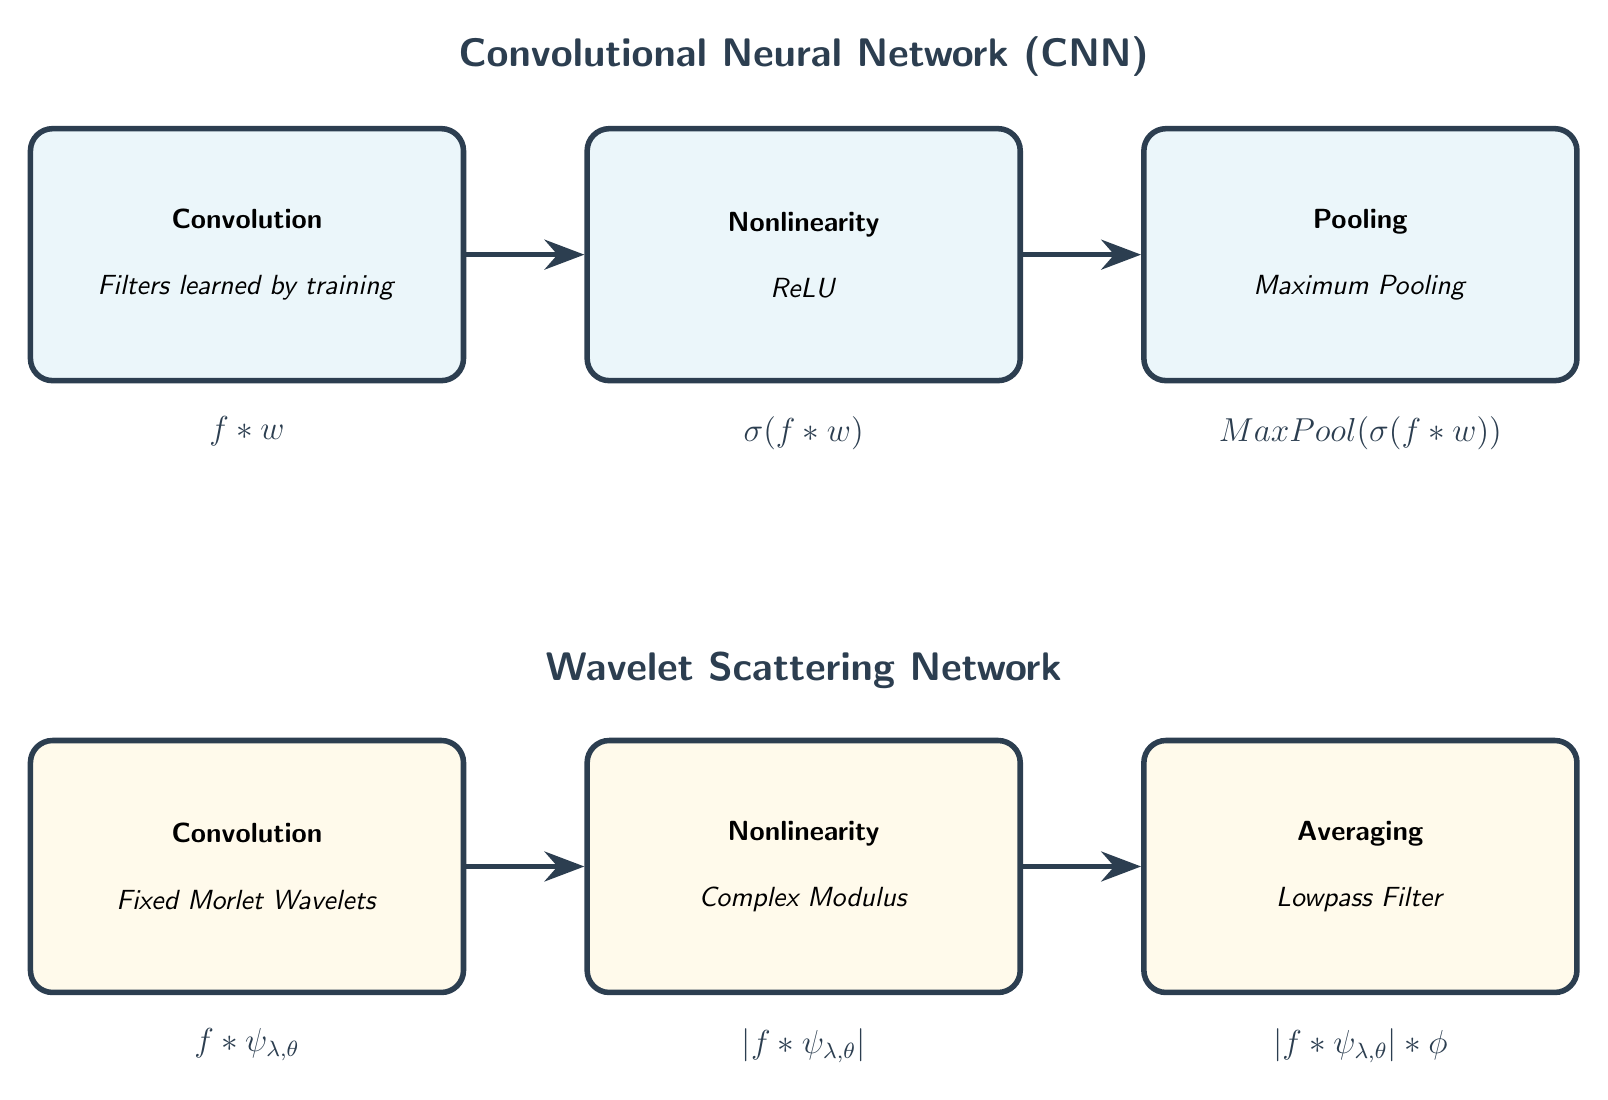
\begin{tikzpicture}[
    node distance=1.5cm and 1.5cm,
    baseblock/.style={
        rectangle,
        rounded corners=8pt,
        draw=darkslate,
        line width=2pt,
        minimum width=5.5cm,
        minimum height=3.2cm,
        align=center,
        font=\sffamily
    },
    cnnblock/.style={baseblock, fill=bgblue},
    wsnblock/.style={baseblock, fill=bgyellow},
    arrowstyle/.style={draw=darkslate, -{Stealth[scale=1.2]}, line width=2pt},
    mathlabel/.style={text=darkslate, font=\large, anchor=north},
    titlelabel/.style={text=darkslate, font=\sffamily\bfseries\Large, align=center}
]

    % --- Row 1: CNN ---

    % Nodes
    \node[cnnblock] (cnn1) {
        \textbf{Convolution}\\[1.2em]
        \textit{Filters learned by training}
    };

    \node[cnnblock, right=of cnn1] (cnn2) {
        \textbf{Nonlinearity}\\[1.2em]
        \textit{ReLU}
    };

    \node[cnnblock, right=of cnn2] (cnn3) {
        \textbf{Pooling}\\[1.2em]
        \textit{Maximum Pooling}
    };

    % Title
    \node[titlelabel, above=0.5cm of cnn2] {Convolutional Neural Network (CNN)};

    % Math Labels
    \node[mathlabel] at (cnn1.south) [yshift=-0.3cm] {$f * w$};
    \node[mathlabel] at (cnn2.south) [yshift=-0.3cm] {$\sigma(f * w)$};
    \node[mathlabel] at (cnn3.south) [yshift=-0.3cm] {$MaxPool(\sigma(f * w))$};

    % Arrows
    \draw[arrowstyle] (cnn1) -- (cnn2);
    \draw[arrowstyle] (cnn2) -- (cnn3);


    % --- Row 2: WSN ---

    % Nodes (positioned relative to top row for alignment)
    \node[wsnblock, below=4.5cm of cnn1] (wsn1) {
        \textbf{Convolution}\\[1.2em]
        \textit{Fixed Morlet Wavelets}
    };

    \node[wsnblock, right=of wsn1] (wsn2) {
        \textbf{Nonlinearity}\\[1.2em]
        \textit{Complex Modulus}
    };

    \node[wsnblock, right=of wsn2] (wsn3) {
        \textbf{Averaging}\\[1.2em]
        \textit{Lowpass Filter}
    };

    % Title
    \node[titlelabel, above=0.5cm of wsn2] {Wavelet Scattering Network};

    % Math Labels
    \node[mathlabel] at (wsn1.south) [yshift=-0.3cm] {$f * \psi_{\lambda, \theta}$};
    \node[mathlabel] at (wsn2.south) [yshift=-0.3cm] {$|f * \psi_{\lambda, \theta}|$};
    \node[mathlabel] at (wsn3.south) [yshift=-0.3cm] {$|f * \psi_{\lambda, \theta}|*\phi$};

    % Arrows
    \draw[arrowstyle] (wsn1) -- (wsn2);
    \draw[arrowstyle] (wsn2) -- (wsn3);

\end{tikzpicture}
\end{document}